\section{Wheeled Vehicle Kinematics}
This section is about how coordinate frames move according the geometry, velocities, rotational rates, positions and orientations of their mechanical elements. The section puts the focus on  different configurations of wheeled vehicles. The goal of each subsection is to find out the relation between the actuators (usually wheel rotation rates and/or steering angles) and the kinematic state of the vehicle, which is usually a 2D twist $(v_x, v_y, w_z)$, corresponding to forward velocity, lateral velocity and rotational rate respectively. To simplify the notation, this 2D twist will be written as $(u, v, w)$ through this section. 

\subsection{Forward and inverse kinematics}
Two relations are of interest between actuators and vehicle twist: \textit{forward} and \textit{inverse} kinematics. 

Forward kinematics gets actuator values as inputs and computes the twist, while inverse kinematics computes the actuator values given a twist as input. The former is generally of interest in estimation and prediction problems, while the later is usually of interest in planning and control. 

\subsection{The Coriolis Law}
Given two coordinate frames, one called \textit{moving}($\mathcal{F}^M$) which is rotating at angular velocity~$\mathbf{w}$ about the other frame, called \textit{fixed}($\mathcal{F}^F$). Then the derivative of any vector $\mathbf{x}$ with respect to the time is related by: 
\begin{equation}
\label{eq:coriolis}
 \frac{d\mathbf{x}^F}{dt} = \frac{d\mathbf{x}^M}{dt} + \mathbf{w} \times  \mathbf{x}^F
\end{equation}
where~$\mathbf{x}$ can be , for instance, position, velocity or force. 

In the practical situation of a vehicle rotating about a fixed frame of reference, a given point~$\mathbf{p}$ of that vehicle (fixed with respect to the vehicle frame) has a null time derivative in the vehicle frame ($\frac{d\mathbf{p}^M}{dt} = 0$), so equation~\ref{eq:coriolis} simplifies to the expression of the linear velocity of any point of the vehicle according to the rotation of the vehicle and the position of that point with respect to fixed frame.
\begin{equation}
 \mathbf{v} = \frac{d\mathbf{p}^F}{dt} = \mathbf{w} \times \mathbf{p}^F
\end{equation}


\subsection{Instantaneous Center of Rotation (ICR)}
From mechanics, we know that all planar motions of a rigid body can be described as a pure rotation about some point, called the instantaneous center of rotation (ICR). All points of the rigid body can describe its motion as a rotation about the same ICR. 

For kinematics analysis, it is of special interest the contact point of the wheels with the floor, since these points are fixed in the vehicle frame and they also have the wheel restriction of no slippage. 


\subsection{Single Wheel}
\label{subsec:single_wheel}
The most basic mechanical element of wheeled vehicles are their wheels, so let's take a look on how they work from the kinematics point of view.

A wheel is actuated with a motor providing a rotation rate to its axis, $\Omega$. This rotation rate, will cause a linear velocity of the wheel center as: 
\begin{equation}
 u = \Omega r
\end{equation}
where $r$ is the wheel radius. 

Despite forward velocity, a single wheel has $v = w = 0$, since it is not actuated to cause motion other than forward (1D case). It is a straightforward example of how the geometry of a body shapes the relation between the actuation variable (rotational rate, $\Omega$), and the derived state of the `vehicle` (linear velocity, $u$)


\subsection{Bicycle}
\label{subsec:bicycle}
The bicycle case is the platform composed by two wheels mounted one in front of the other, separated by a distance $L$. The rear wheel drives the vehicle, while the front one steers it. Figure~\ref{fig:bike_kinematics} shows this configuration.
\begin{figure}[bth!]
  \begin{center}
    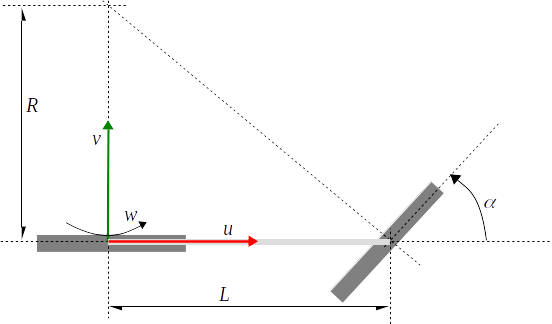
\includegraphics[width=1.0\columnwidth]{figures/bike_kinematics.png}
    \caption{Bicycle configuration.}
    \label{fig:bike_kinematics}
  \end{center}
\end{figure}
Actuator inputs are rear wheel rotation rate, $\Omega$, and front wheel steering angle, $\alpha$. Constructive parameters are the distance between wheels ,$L$, and the rear wheel radius, $r$. Parameter $R$ in the figure~\ref{fig:bike_kinematics} is the curvature radius, which is an intermediate parameter of ineterst.

The linear velocities are: 
\begin{align}
\label{eq:bike_fwd_kinematics_1}
u = \Omega r \\
v = 0
\end{align} 
and the vehicle should fulfill:
\begin{equation}
 u = wR.
\end{equation}
Given 
\begin{equation}
 \tan \alpha = \frac{L}{R}
\end{equation}
and matching the two previous expressions for $u$:
\begin{equation}
 u = \Omega r = wR = w\frac{L}{\tan \alpha} 
\end{equation}
leads to the expression for vehicle rotation rate: 
\begin{equation}
\label{eq:bike_fwd_kinematics_2}
w=\frac{\Omega r}{L} \tan \alpha 
\end{equation}

In this case the forward kinematics is not linear, since the $w$ part of the twist involve a $\tan()$ relation with the input parameter $\alpha$. 

For several purposes it might be interesting to linearize this relation between input actuators, constructive parameters and output twist(see section~\ref{sec:Linearization} for linearization overview). Starting with the linearization with respect to the input actuators~$\alpha$ and~$\Omega$, the Jacobian is: 
\begin{equation}
\mathbf{J}_{\alpha \Omega} = 
\left[
 \begin{array}{cc}
  0 & r  \\
  0 & 0  \\
  \frac{\Omega r}{L \cos ^2 \alpha} & \frac{r}{L}\tan \alpha
 \end{array}
 \right]; \\ 
\end{equation}
 so forward kinematics relation can be approximated by the linearization as follows: 
\begin{equation}
 \left[
 \begin{array}{c}
  u \\
  v  \\
  w 
 \end{array}
 \right] \approx \mathbf{J}_{\alpha \Omega}
 \left[
 \begin{array}{c}
  \alpha \\
  \Omega \\
 \end{array} 
 \right]
\end{equation}
which can be useful, for instance, for Kalman filtering (see section~\ref{sec:KalmanFilter}).

If the interest is to analyze how sensitive is the kinematics to the constructive parameters, the goal is to compute the Jacobian matrix with respect to the parameters~$r$ and~$L$, and perform an error propagation analysis. First the linearized relation is: 
\begin{equation}
\mathbf{J}_{r L} = 
\left[
 \begin{array}{cc}
  \Omega & 0  \\
  0 & 0  \\
  \frac{\Omega}{L}\tan \alpha & -\frac{\Omega r}{L^2}\tan \alpha
 \end{array}
 \right]; \\ 
\end{equation}
Given an uncertainty in the ~$r$ and~$L$ parameters, represented with a covariance matrix as:
\begin{equation}
\mathbf{C}_{r L} = 
\left[
 \begin{array}{cc}
  \sigma^2_r & 0  \\
  0 & \sigma^2_L  \\
 \end{array}
 \right]; \\ 
\end{equation}
the propagation of such uncertainty to twist space is: 
\begin{equation}
\mathbf{C}_{uvw} = \mathbf{J}_{r L} \mathbf{C}_{r L} \mathbf{J}_{r L}^T = 
 \left[
 \begin{array}{cc}
  \Omega & 0  \\
  0 & 0  \\
  \frac{\Omega}{L}\tan \alpha & -\frac{\Omega r}{L^2}\tan \alpha
 \end{array}
 \right]
 \left[
 \begin{array}{cc}
  \sigma^2_r & 0  \\
  0 & \sigma^2_L  \\
 \end{array}
 \right]
 \left[
 \begin{array}{ccc}
  \Omega & 0 & \frac{\Omega}{L}\tan \alpha\\
  r & 0 & -\frac{\Omega r}{L^2}\tan \alpha
 \end{array}
 \right];
\end{equation}
\begin{equation}
\mathbf{C}_{uvw} = 
 \left[
 \begin{array}{ccc}
  \sigma^2_r \Omega^2 & 0 & \sigma^2_r \frac{\Omega^2}{L}\tan \alpha\\
  0 & 0 & 0\\
  \sigma^2_r \frac{\Omega^2}{L}\tan \alpha & 0 & \frac{\Omega^2}{L^2}\tan^2 \alpha (\sigma^2_r+\frac{r^2}{L^2} \sigma^2_L )
 \end{array}
 \right];
\end{equation}
Meaning that for a reasonable uncertainty values of $\sigma^2_r=10^{-6}\ m^2$ and $\sigma^2_L=10^{-6}\ m^2$ ($1\ mm$ of standard deviation in both cases~$r$ and~$L$), and evaluating at~$\Omega=2\pi\ rad/s$,~$\alpha=45^o$,~$r=0.4\ m$ and~$L=1\ m$, the standard deviations in linear speed and rotational rate of the vehicle are: 
\begin{equation}
 \sigma_u \approx 6\ mm/s ; \ \ \ \sigma_w \approx 4\ mrad/s ;
\end{equation}


\paragraph{Inverse kinematics}
Inverse kinematics for the bicycle configuration is found from equations~\ref{eq:bike_fwd_kinematics_1} and~\ref{eq:bike_fwd_kinematics_2} as follows: 
\begin{align}
 \Omega & = \frac{u}{r} \\
 \alpha & = \arctan(L\frac{w}{u}), \ \ \alpha \in [-\pi/2,\pi/2]
\end{align}


\subsection{Tricycle}
The tricycle has two configurations, depending if the drive actuator is at the front axis or at the back one. In the former configuration, the kinematics relation is exactly those previously analyzed for the monocycle case. However, in the later configuration, the driving actuator is attached at the rear axis, providing a forward velocity, while the front wheel just steers the vehicle. So, this configuration is like the bicycle case analyzed above, but some extra differential mechanism is required to drive each rear wheel at different speeds when turning, otherwise the wheels would slip. 


\subsection{Two wheels differential drive}
Two wheels differential drive configuration is an essential and widely used architecture, due to its building simplicity and good manoeuvring properties, since it allows the platform to turn on the spot. 

Figure~\ref{fig:differential_kinematics} shows the two wheels differential drive configuration as well as the involved parameters and variables. 
\begin{figure}[bth!]
  \begin{center}
    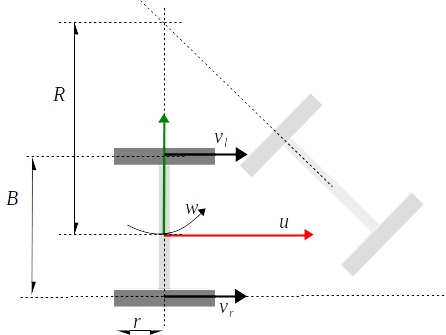
\includegraphics[width=1.0\columnwidth]{figures/differential_kinematics.png}
    \caption{Two wheels differential drive configuration.}
    \label{fig:differential_kinematics}
  \end{center}
\end{figure}

Actuator inputs are left and right wheel rotation rates, $\Omega_l, \Omega_r$. Constructive parameters are the baseline distance between wheels ,$B$, and the wheel radius, $r$. Parameter $R$ in the figure~\ref{fig:differential_kinematics} is the curvature radius, which is an intermediate parameter of ineterst.

Placing the platform frame at the mid point on the baseline joining the wheels, we define the twist of this frame as $(u, v, w)$. Applying the Coriolis principle, three equations are deduced, for the left wheel center point, the right wheel center point and the vehicle origin, respectively:
\begin{align}
v_l = & \Omega_l r = w(R-\frac{B}{2}) \\
v_r = & \Omega_r r = w(R+\frac{B}{2}) \\
u = & wR \\
\end{align} 
operating on $v_r-v_l$, leads to:
\begin{equation}
\label{eq:diff_drive_fwd_kinematics_w}
w = \frac{v_r-v_l}{B}
\end{equation}
and solving for $v_r+v_l$, the linear forward velocity is:  
\begin{equation}
\label{eq:diff_drive_fwd_kinematics_u}
u = \frac{v_r+v_l}{2}
\end{equation}

In this case the kinematics relation between actuators and platform twist is linear, and can be written in the matrix form:
\begin{equation}
\label{eq:diff_drive_fwd_kinematics_matrix}
 \left[
 \begin{array}{c}
  u \\
  w \\
 \end{array}
 \right] = 
 \left[
 \begin{array}{cc}
  \frac{1}{2} & \frac{1}{2} \\
  -\frac{1}{B} & \frac{1}{B} \\
 \end{array}
 \right]
 \left[
 \begin{array}{c}
  v_l \\
  v_r \\
 \end{array}
 \right] = 
 \left[
 \begin{array}{cc}
  \frac{r}{2} & \frac{r}{2} \\
  -\frac{r}{B} & \frac{r}{B} \\
 \end{array}
 \right]
 \left[
 \begin{array}{c}
  \Omega_l \\
  \Omega_r \\
 \end{array}
 \right]
\end{equation}

As in the bicycle case (see subsection \ref{subsec:bicycle}), we might be interested how errors on constructive parameters~$r$ and~$B$ propagate to the platform twist. In this case the Jacobian of the twist with respect to these parameters is computed as: 
\begin{equation}
\mathbf{J}_{r B} = 
\left[
 \begin{array}{cc}
  \frac{1}{2}(\Omega_r+\Omega_l) & 0  \\
  \frac{1}{B}(\Omega_r-\Omega_l) & \frac{r}{B^2}(\Omega_l-\Omega_r)  \\
 \end{array}
 \right]; \\ 
\end{equation}
Given an uncertainty in the ~$r$ and~$B$ parameters, represented with a covariance matrix as:
\begin{equation}
\mathbf{C}_{r B} = 
\left[
 \begin{array}{cc}
  \sigma^2_r & 0  \\
  0 & \sigma^2_B  \\
 \end{array}
 \right]; \\ 
\end{equation}
the propagation of such uncertainty to twist space is: 
\begin{equation}
\mathbf{C}_{uw} = \mathbf{J}_{r B} \mathbf{C}_{r B} \mathbf{J}_{r B}^T = 
 \left[
 \begin{array}{cc}
 \frac{\sigma^2_r}{4}(\Omega_r+\Omega_l)^2 & \frac{\sigma^2_r}{4}(\Omega_r+\Omega_l)(\Omega_r-\Omega_l) \\
 \frac{\sigma^2_r}{4}(\Omega_r+\Omega_l)(\Omega_r-\Omega_l) & \frac{\sigma^2_r}{4}(\Omega_r-\Omega_l)^2 + \frac{\sigma^2_B r^2}{B^4}(\Omega_l-\Omega_r)^2 \\
 \end{array}
 \right];
 \label{eq:differential_twist_uncertainty}
\end{equation}
Result in equation~\ref{eq:differential_twist_uncertainty} suggests that error in baseline length~$B$ only affects the uncertainty of the platform rotation rate, while errors in wheel radius~$r$ propagates to both components of the twist~$u$ and ~$w$. 

\paragraph{Inverse kinematics}
Inverse kinematics for the two wheels differential configuration can be derived by inverting the linear model in equation~\ref{eq:diff_drive_fwd_kinematics_matrix}, or from equations~\ref{eq:diff_drive_fwd_kinematics_u} and~\ref{eq:diff_drive_fwd_kinematics_w}: 
\begin{align}
\label{eq:diff_drive_inv_kinematics}
 v_r & = u + w\frac{B}{2} \\
 v_l & = u - w\frac{B}{2} \\
\end{align}
which suggests that for positive rotations, the right wheel should turn faster than the left one.

\subsection{4 wheels differential drive}
At kinematics level, this configuration reduces to the case of two wheel differential drive since both left wheels have the same rotation rate and both right wheels have also the same rotation rate. However, when the vehicle is rotating, null lateral velocity at wheels is no longer fulfilled, so the wheels slip when turning. 


\subsection{Ackermann}
Ackermann system is the standard steering for most of the nowadays cars and trucks. Figure~\ref{fig:ackermann_kinematics} shows the steering mechanism, the constructive parameters~$B$ and~$L$ and the input actuators~$\alpha$ and~$u$, the later being directly the forward velocity to be transmitted to each rear wheel.  
\begin{figure}[bth!]
  \begin{center}
    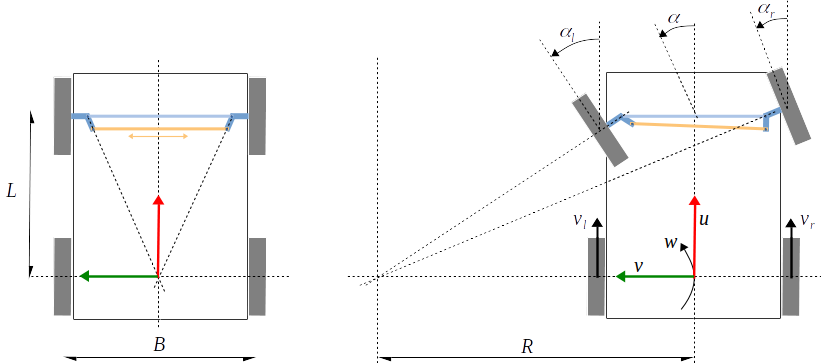
\includegraphics[width=1.0\columnwidth]{figures/ackermann_kinematics.png}
    \caption{Ackermann configuration. Steering is achieved by actuating the orange bar.  }
    \label{fig:ackermann_kinematics}
  \end{center}
\end{figure}

The kinematics of the Ackermann configuration is reduced to the kinematics of the bike seen at subsection~\ref{subsec:bicycle}, with input actuators~$\alpha$ and~$u$, and constructive parameter~$L$.

However, the Ackermann mechanism ensures a relation between the three steering angles~$\alpha_l$, $\alpha_r$ and~$\alpha$. Given an steering angle~$\alpha$, the tangent of the three triangles with vertex at ICR are: 
\begin{align}
\tan \alpha_l = & \frac{L}{R-\frac{B}{2}} \\
\tan \alpha = & \frac{L}{R} \\
\tan \alpha_r = & \frac{L}{R+\frac{B}{2}} 
\end{align} 
Solving for~$R$ at each equation leads to the following relation that Ackemrann steering should fulfill: 
\begin{align}
\tan \alpha_l = & \frac{1}{\frac{1}{\tan \alpha} - \frac{B}{2L}} \\
\tan \alpha_r = & \frac{1}{\frac{1}{\tan \alpha} + \frac{B}{2L}} \\\end{align} 
which is of interest in case of electronic Ackermann steering. 

Even if forward velocity~$u$ is transmitted to each rear wheel,  velocities of each of these wheels are different and constrained with the vehicle twist. Usually a differential mechanism implements this difference of speeds, but an electronic implementation may implement that, fulfilling the following: 
\begin{align}
v_l = & w(R-\frac{B}{2}) \\
v_r = & w(R+\frac{B}{2})
\end{align} 
which as it has been seen with the two wheel differential drive at equations~\ref{eq:diff_drive_inv_kinematics}, it leads to: 
\begin{align}
v_l = & u -w\frac{B}{2} \\
v_r = & u + w\frac{B}{2}
\end{align} 



\subsection{Double Ackermann}
Double Ackermann configuration refers to those vehicles having an Ackermann steering system (mechanical or electronical) for front and back wheels, actuating both with the same steering angle, so the ICR point is no longer at the line joining rear wheels , but it is at the line parallel to that but passing through the center of the vehicle. This allows such vehicles to make sharper turns than single Ackermann steering configurations. The configuration of double Ackermann steering can be reduced to a bicycle with  steering at front and back wheels, as shown in figure~\ref{fig:double_ackermann_kinematics}.
\begin{figure}[bth!]
  \begin{center}
    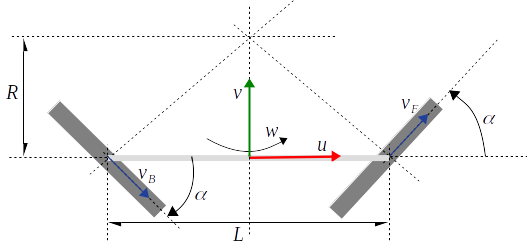
\includegraphics[width=1.0\columnwidth]{figures/double_ackermann_kinematics.png}
    \caption{Double Ackermann configuration can be reduced to the double steering bike.}
    \label{fig:double_ackermann_kinematics}
  \end{center}
\end{figure}

The analysis of this double steering bicycle starts by applying the Coriols principle at the center of each wheel, as well as at the center of the bicycle:
\begin{align}
\mathbf{v_B} = & 
\left[
 \begin{array}{c}
  0  \\
  0  \\
  w 
 \end{array}
\right]
\times 
\left[
 \begin{array}{c}
  -\frac{L}{2}  \\
  -R  \\
  0 
 \end{array}
\right]
= 
\left[
 \begin{array}{c}
  wR  \\
  -w\frac{L}{2}  \\
  0 
 \end{array}
\right] \\
\mathbf{u} = & 
\left[
 \begin{array}{c}
  0  \\
  0  \\
  w 
 \end{array}
\right]
\times 
\left[
 \begin{array}{c}
  0  \\
  -R  \\
  0 
 \end{array}
\right]
= 
\left[
 \begin{array}{c}
  wR  \\
  0  \\
  0 
 \end{array}
\right] \\
\mathbf{v_F} = & 
\left[
 \begin{array}{c}
  0  \\
  0  \\
  w 
 \end{array}
\right]
\times 
\left[
 \begin{array}{c}
  \frac{L}{2}  \\
  -R  \\
  0 
 \end{array}
\right]
= 
\left[
 \begin{array}{c}
  -wR  \\
  w\frac{L}{2}  \\
  0 
 \end{array}
\right]
\end{align} 
The above velocity vectors~$\mathbf{v_B}$, $\mathbf{u}$ and~$\mathbf{v_F}$ are expressed with respect to a frame placed at ICR and aligned with the vehicle frame, so the same velocity vectors are also with respect to the vehicle frame (since there is no rotation between these two frames). For the back wheel, in 2D, we have: 
\begin{equation}
\mathbf{v_B} = 
\left[
 \begin{array}{c}
  wR  \\
  -w\frac{L}{2} 
 \end{array}
\right]
=
|\mathbf{v_B}|
\left[
 \begin{array}{c}
  \cos \alpha  \\
  \sin \alpha
 \end{array}
\right]
=
\Omega_Br
\left[
 \begin{array}{c}
  \cos \alpha  \\
  \sin \alpha
 \end{array}
\right]
\end{equation}
so we can find $R$ and $w$ as: 
\begin{align}
 R = & \frac{\Omega_B r}{w}\cos \alpha \\
 w = & \frac{2\Omega_B r}{L}\sin \alpha \\
\end{align}
and then, with the expression of $\mathbf{u}=\left[u_x\ u_y \right]^T$ in 2D: 
\begin{equation}
 u_x = wR = \Omega_Br \cos \alpha \ ; \ \ u_y = 0; 
\end{equation}

A practical case of double Ackermann steering (or even more than double!) is the straddle carrier family (see figure~\ref{fig:straddle_carrier}), which are large vehicles that need to manoeuver usually in tight spaces with respect to their dimensions~$L$ and~$B$. 
\begin{figure}[bth!]
  \begin{center}
    \includegraphics[width=0.6\columnwidth]{figures/straddle_carrier.jpg}
    \caption{Straddle carriers are big vehicles that need to perform good manoeuvring, so they have double (or even quadruple like in this picture) Ackermann steering, usually implemented with electronic/software means instead of by a mechanism.}
    \label{fig:straddle_carrier}
  \end{center}
\end{figure}


\subsection{Holonomic wheels}
Holonomic wheels refers to those wheels that have an extra set of small rollers mounted with their axis forming an angle $\gamma$ with the wheel perpendicular direction of driving. This angle $\gamma$ is usually $0$~degrees for \textit{omniwheels} or $45$~degrees for \textit{mecanum} wheels. These rollers allow the wheel to freely move in lateral motion, while keeping the actuated forward (standard) motion of a wheel, so the constraint of null lateral motion described in~\ref{subsec:single_wheel} no longer fulfills. 

Figure\ref{fig:omniwheel_kinematics} shows the involved frames and vectors to analyze the inverse kinematics of an omniwheel mounted in a vehicle frame.
\begin{figure}[bth!]
  \begin{center}
    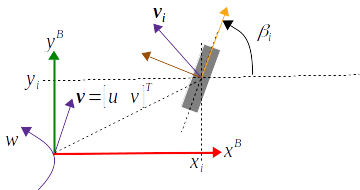
\includegraphics[width=1.0\columnwidth]{figures/omniwheel_kinematics.png}
    \caption{Frames and vectors involved in the omniwheel kinematcs analysis. Vehicle frame in green and red. In yellow wheel driving direction and in brown wheel free sliding direction for omniwheels. }
    \label{fig:omniwheel_kinematics}
  \end{center}
\end{figure}

Given a vehicle twist~$[u v w]$, the procedure will find the inverse kinematics model, so the required wheel angular speeds for each wheel. The first step is to find the linear velocity of the wheel center with respect to the vehicle base frame~$\mathcal{F}^B$, given the vehicle twist, by applying the Coriolis law: 
\begin{equation}
\mathbf{v^B_i} = 
\left[
 \begin{array}{c}
  u  \\
  v \\
  0
 \end{array}
\right]
+
\left[
 \begin{array}{c}
  0  \\
  0 \\
  w
 \end{array}
\right]
\times
\left[
 \begin{array}{c}
  x_i \\
  y_i
 \end{array}
\right] 
= 
\left[
 \begin{array}{c}
  u  \\
  v \\
  0
 \end{array}
\right]
+
\left[
\begin{array}{c}
 -w y_i \\
 w x_i \\
 0
\end{array}
\right] 
= 
\left[
\begin{array}{ccc}
 1 & 0 & -y_i \\
 0 & 1 &  x_i 
\end{array}
\right] 
\left[
\begin{array}{c}
 u \\
 v \\
 w
\end{array}
\right] 
\end{equation}

Once we know the wheel center linear speed with respect to the vehicle frame, we will transform it to the wheel frame by applying the rotation (only the 2D part): 
\begin{equation}
\mathbf{v^{W}_i} = 
\left[
 \begin{array}{cc}
  \cos \beta_i & \sin \beta_i  \\
  -\sin \beta_i & \cos \beta_i \\
 \end{array}
\right]
\left[
\begin{array}{ccc}
 1 & 0 & -y_i \\
 0 & 1 &  x_i 
\end{array}
\right] 
\left[
\begin{array}{c}
 u \\
 v \\
 w
\end{array}
\right] 
\end{equation}

Finally, from~$\mathbf{v^{W}_i}$, we only take the first component, which is the actuated velocity (aligned with the wheel driving direction): 
\begin{equation}
u_i
=
\left[
\begin{array}{cc}
 1 & 0
\end{array}
\right]
\left[
 \begin{array}{cc}
  \cos \beta_i & \sin \beta_i  \\
  -\sin \beta_i & \cos \beta_i \\
 \end{array}
\right]
\left[
\begin{array}{ccc}
 1 & 0 & -y_i \\
 0 & 1 &  x_i 
\end{array}
\right] 
\left[
\begin{array}{c}
 u \\
 v \\
 w
\end{array}
\right] 
\end{equation}
which can be simplified to: 
\begin{equation}
u_i 
=
\left[
\begin{array}{ccc}
 \cos \beta_i & \sin \beta_i & -y_i\cos \beta_i+x_i \sin \beta_i
\end{array}
\right]
\left[
\begin{array}{c}
 u \\
 v\\
 w
\end{array}
\right]
\label{eq:single_omniwheel_inverse_kniematics}
\end{equation}

A vehicle with $N$ omniwheels (at least $N=3)$, will stack $N$ equations that constraint the actuated wheel angular speeds given the vehicle twist. The following subsections analyses the cases for $N=3$ and $N=4$. 


\subsection{4 omniwheels}
The four omniwheels configuration is a rather standard platform allowing high manoeuvrability and stability. Figure~\ref{fig:four_omniwheels_kinematics} shows this configuration when mounted in a squared platform of side size $2L$.
\begin{figure}[bth!]
  \begin{center}
    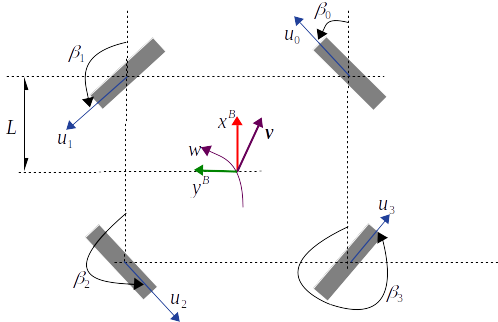
\includegraphics[width=1.0\columnwidth]{figures/four_omniwheels_kinematics.png}
    \caption{Configuration for a platform with four omniwheels in a square base of side size $2L$.}
    \label{fig:four_omniwheels_kinematics}
  \end{center}
\end{figure}

Table~\ref{tab:params_4_omni} details the constructive parameters~$x_i,y_i,B_i$ for this vehicle. 
\begin{table}[hbt] \centering
\caption{Constructive parameters for squared 4-omniwheel vehicle of side size $2L$}
\begin{tabular}
[c]{|c|c|c|c|}\hline
		& $x_i$ 		& $y_i$				& $\beta_i$ \\\hline
Wheel 0 & $L$ 		    & $-L$				& $\pi/4$ \\\hline
Wheel 1 & $L$ 		    & $L$				& $3\pi/4$ \\\hline
Wheel 2 & $-L$ 		    & $L$				& $5\pi/4$ \\\hline
Wheel 3 & $-L$ 		    & $-L$				& $7\pi/4$ \\\hline
\end{tabular}
\label{tab:params_4_omni}
\end{table}

With the constructive parameters, wheel actuated speeds can be computed by applying equation~\ref{eq:single_omniwheel_inverse_kniematics} for each wheel ($i=0,..,3$):
\begin{equation}
\left[
\begin{array}{c}
u_0 \\
u_1 \\
u_2 \\
u_3 \\
\end{array}
\right]
=
\left[
\begin{array}{ccc}
 \cos \beta_0 & \sin \beta_0 & -y_0\cos \beta_0+x_0 \sin \beta_0 \\
 \cos \beta_1 & \sin \beta_1 & -y_1\cos \beta_1+x_1 \sin \beta_1 \\
 \cos \beta_2 & \sin \beta_2 & -y_2\cos \beta_2+x_2 \sin \beta_2 \\
 \cos \beta_3 & \sin \beta_3 & -y_3\cos \beta_3+x_3 \sin \beta_3 \\
\end{array}
\right]
\left[
\begin{array}{c}
 u \\
 v\\
 w
\end{array}
\right], 
\end{equation}

so the full inverse kinematics results as follows: 
\begin{equation}
\left[
\begin{array}{c}
u_0 \\
u_1 \\
u_2 \\
u_3 \\
\end{array}
\right]
=
\left[
\begin{array}{ccc}
 \frac{1}{\sqrt{2}} & \frac{1}{\sqrt{2}} & L\sqrt{2} \\
 -\frac{1}{\sqrt{2}} & \frac{1}{\sqrt{2}} & L\sqrt{2} \\
 -\frac{1}{\sqrt{2}} & -\frac{1}{\sqrt{2}} & L\sqrt{2} \\
 \frac{1}{\sqrt{2}} & -\frac{1}{\sqrt{2}} & L\sqrt{2} \\
\end{array}
\right]
\left[
\begin{array}{c}
 u \\
 v\\
 w
\end{array}
\right], 
\end{equation}

Please remind that $u_i$ are the linear speeds of wheel centers in the driving direction. To find the angular speed of the wheel we have to apply $\Omega_i = u_i/r$, where $r$ is the radius of the wheel. 


\subsection{3 omniwheels}
A typical configuration using omniwheels is also that of mounting three of them in an equilateral triangle base, as depicted in figure~\ref{fig:three_omniwheels_kinematics}.
\begin{figure}[bth!]
  \begin{center}
    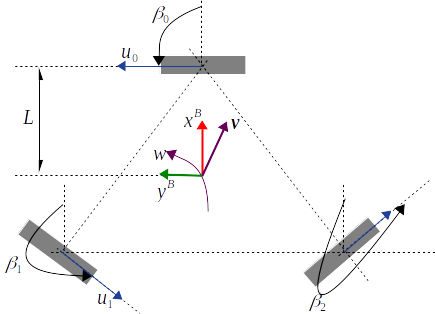
\includegraphics[width=1.0\columnwidth]{figures/three_omniwheels_kinematics.png}
    \caption{Configuration for a platform with three omniwheels in an equilateral triangle.}
    \label{fig:three_omniwheels_kinematics}
  \end{center}
\end{figure}

In this case table~\ref{tab:params_3_omni} shows the constructive parameters  $x_i,y_i,\beta_i$: 
\begin{table}[hbt] \centering
\caption{Constructive parameters for triangular 3-omniwheel vehicle of side size $2L$}
\begin{tabular}
[c]{|c|c|c|c|}\hline
		& $x_i$ 		    & $y_i$				& $\beta_i$ \\\hline
Wheel 0 & $L$ 		        & $0$				& $3\pi/6$ \\\hline
Wheel 1 & $-L\sin(\pi/6)$   & $L\cos(\pi/6)$	& $7\pi/6$ \\\hline
Wheel 2 & $-L\sin(\pi/6)$ 	& $-L\cos(\pi/6)$	& $11\pi/4$ \\\hline
\end{tabular}
\label{tab:params_3_omni}
\end{table}

Therefore, applying equation~\ref{eq:single_omniwheel_inverse_kniematics}, the inverse kinematics results in the following: 
\begin{equation}
\left[
\begin{array}{c}
u_0 \\
u_1 \\
u_2 \\
\end{array}
\right]
=
\left[
\begin{array}{ccc}
 0      & 1     & L \\
-\frac{\sqrt{3}}{2} & -\frac{1}{2} & L \\
 \frac{\sqrt{3}}{2} & -\frac{1}{2} & L \\
\end{array}
\right]
\left[
\begin{array}{c}
 u \\
 v \\
 w
\end{array}
\right]
\end{equation}



\subsection{4 mecanum wheels}


\subsection{Dynamics}


